\section{Grundlagen des Text Mining}\raggedbottom
Im nachfolgenden Kapitel werden jene Konzepte des \textit{Text Minings} erläutert, welche grundlegend für das Verständnis von Methoden der Textklassifikation sind. Abbildung \ref{pipetk} zeigt die Phasen, die beginnend beim Textkorpus (Sammlung der Ausgangstexte) bis zur abschließenden Einstufung durchlaufen werden. Hieran werde ich mich bei den Ausführungen orientieren.
\begin{figure}[htb]
	\begin{center}
		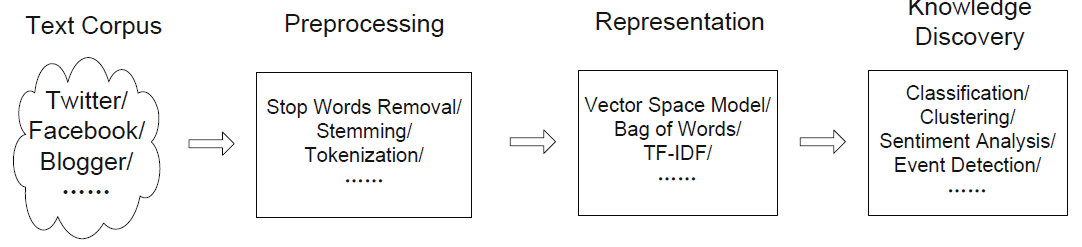
\includegraphics[height=0.25\linewidth, width=0.95\textwidth]{bilder/Abb2.png}
		\caption{Pipeline der Textklassifikation \citep{Kow19}  }\label{pipetk}
	\end{center}
\end{figure}
\subsection{Preprocessing}
Der rohe, unbehandelte Text wird beim \textit{Preprocessing} (deutsch: Vorbehandlung) in eine Form überführt, die eine nachfolgende Repräsentation der Daten durch Vektoren und ähnliche Methoden ermöglicht. Je nach gewünschter Anwendung sind hier verschiedene Vorverarbeitungsverfahren in Betracht zu ziehen.\\
Der Begriff Wortsegmentierung bzw. \textbf{Tokenisierung} bezeichnet die Zerteilung des Ausgangstexts in kleinere Einheiten, sogenannte \textit{Token} \citep{MannSch99}. In der Regel handelt es sich hierbei um einzelne Wörter, Zahlen und Satzzeichen. Als grundsätzliches Abgrenzungszeichen gelten in den meisten Sprachen die \textit{Whitespace}-Zeichen (Leerzeichen, Tab, Newline-Zeichen). Dies wird auch auf die zu analysierenden Tweets zutreffen, da diese fast ausschließlich in englischer Sprache verfasst sind.\\
\begin{figure}[htb]
	\begin{center}
		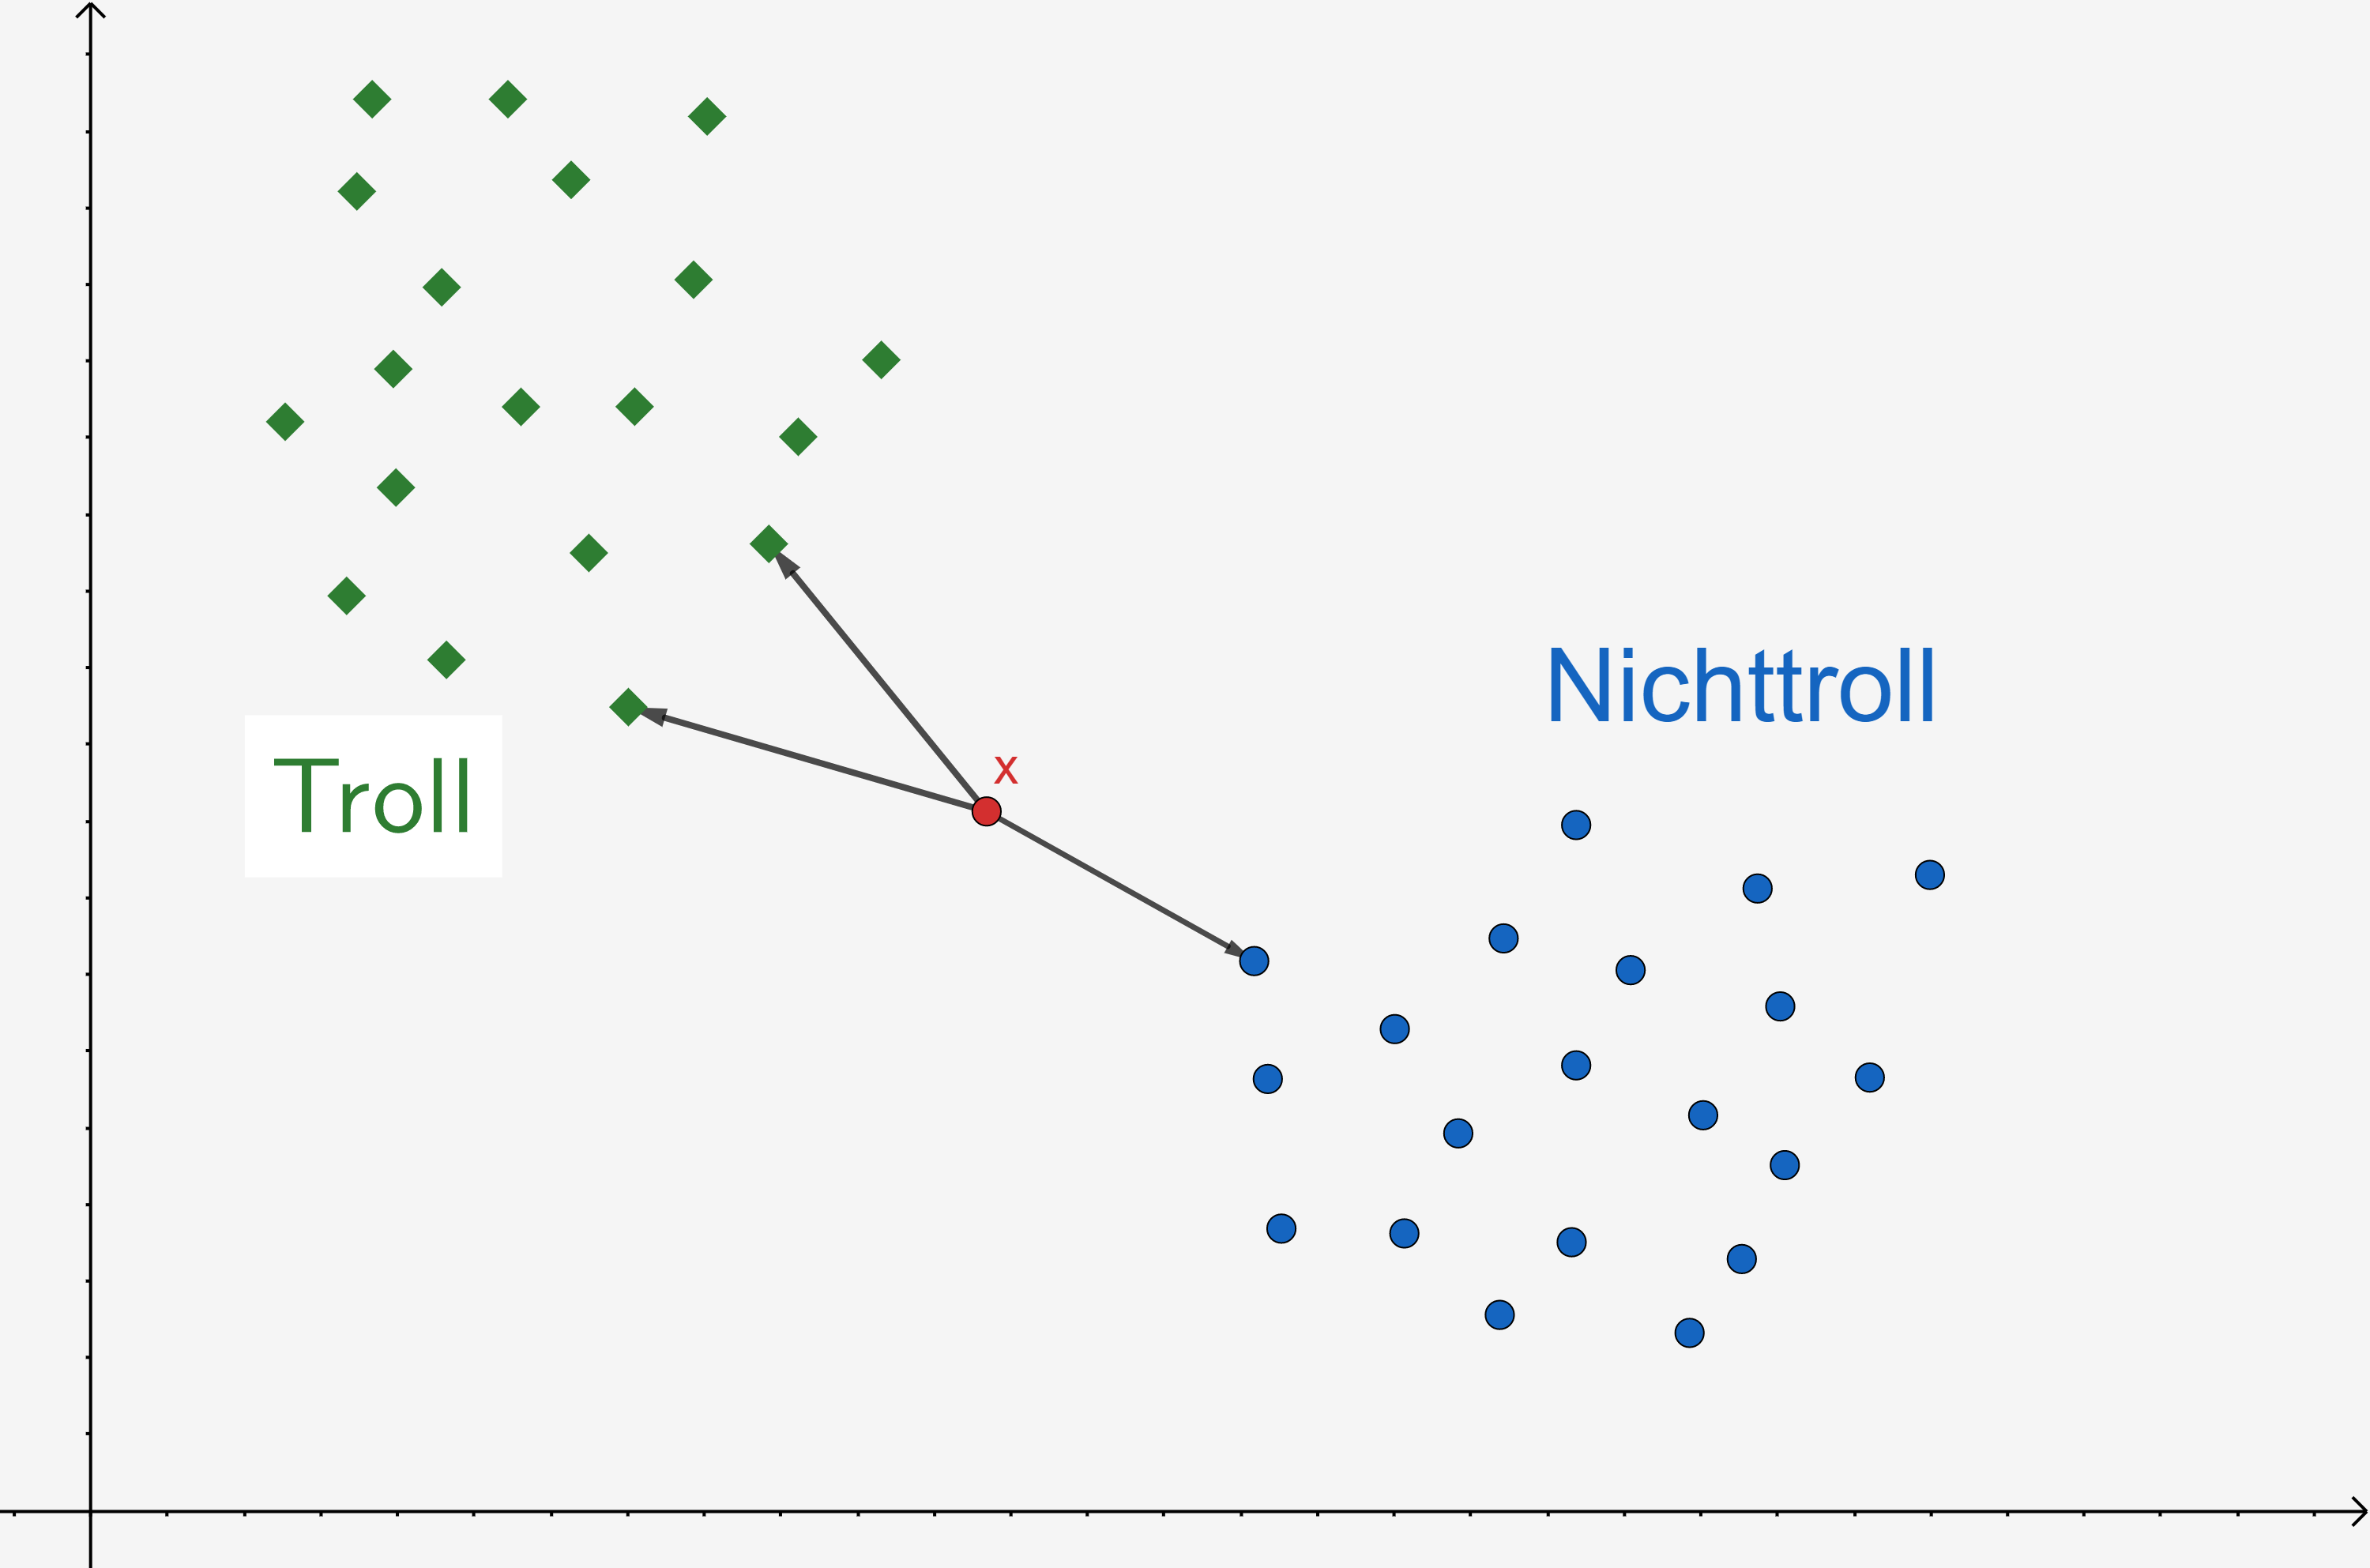
\includegraphics[width=\textwidth]{bilder/Abb3.png}
		\caption{Tokenisierung eines Beispielsatzes}\label{tokenization}
	\end{center}
\end{figure}\\
Eine weitere Methode der Vorverarbeitung ist das Entfernen von \textbf{Stoppwörtern}. Dies sind sehr häufig auftretende Wörter wie \glqq der\grqq, \glqq die\grqq, \glqq das\grqq, \glqq und\grqq{} oder \glqq von\grqq, welche vornehmlich eine grammatikalische Funktion und keine Bedeutung im Sinne von Semantik haben. Ob die Filterung von Stoppwörtern angezeigt ist, hängt vom Anwendungsfall ab. Ein grundsätzlich denkbarer Fall wäre, dass Trolle in ihren Tweets entweder über- oder unterdurchschnittlich Gebrauch von diesen Wörtern machen. Eine Filterung würde dann zu einem Verlust von Unterscheidungsmerkmalen und damit zu einer erschwerten Klassifikation führen. Im Falle dass kein Unterschied zwischen Trollen und Nichttrollen in dieser Eigenschaft besteht, bringt die Filterung durch weniger zu berücksichtigende Token Performanceverbesserungen mit sich.\\
\subsection{Feature Extraction}
Bevor eine Klassifikation vorgenommen werden kann, müssen aus den vorliegenden Texten Merkmale gewonnen werden, welche einen Vergleich im Bezug auf Ähnlichkeit und Unterschiedlichkeit ermöglichen. Die extrahierten Merkmale bilden dann zusammengefasst in einem Merkmalvektor eine eindeutige numerische Repräsentation eines Textes. Die Vektorisierung schafft zudem die Grundlage für verschiedenste Operationen wie Abstandsmessungen, die später bei den Klassifikationsverfahren zum Einsatz kommen werden.\\
Die einfachste Vektorisierungstechnik ist die \textbf{Bag-of-Words} (BoW) \citep{Ramos13}. Hier wird ein Text durch einen Vektor mit den Begriffshäufigkeiten (auch: \textit{Term Frequencies} (\textbf{TF})) aller zuvor extrahierten Tokens des Textkorpus repräsentiert. Bei einem Beispielkorpus mit den beiden Texten \glqq my coffee is too hot\grqq{} und \glqq my tea is too cold\grqq{} und dem zuvor extrahierten Vokabular
\begin{flushleft}
	\hfil\{ "my", "coffee", "hot", "tea", "cold" \}
\end{flushleft}
ergibt sich die folgende Repräsentation:
\begin{flushleft}
	\hfil$v_1$ = [ 1, 1, 1, 0, 0 ]\\
	\hfil$v_2$ = [ 1, 0, 0, 1, 1 ]
\end{flushleft}
Eine Erweiterung dieser TF-Methode ist \textit{Term Frequency-Inverse Document Frequency} (\textbf{TF-IDF}) \citep{Ramos13}.  Hier wird die Vorkommenshäufigkeit anders gewichtet, um dem Aspekt gerecht zu werden, dass einige Begriffe überproportional oft vorkommen. Gleichung \ref{tfidf_weight} zeigt die Gewichtung 
\begin{equation}
	w(d,t) = TF(d,t) \cdot \log \left( \frac{N}{{DF}(t)} \right)
	\label{tfidf_weight}
\end{equation} 
wobei $N$ die Anzahl der Texte im Korpus und ${DF}(t)$ die Anzahl der Texte, welche den Begriff $t$ enthalten, ist.\\
Eine Möglichkeit, Wortkombinationen bzw. bestimmte Formulierungen als Merkmal zu berücksichtigen ist das \textbf{N-Gramm} \citep{Kow19}. Dies ist die Zusammenfassung von $N$ aufeinanderfolgenden Token in einem Text. Folglich handelt es sich bei den Elementen einer Bag of Words um 1-Gramme. Das nachfolgende Beispiel zeigt die Repräsentation des Textes \glqq Hier sehen Sie ein Beispiel.\grqq{} mit 2-Grammen:
\begin{flushleft}
	\hfil \{ \grqq Hier sehen \grqq, \grqq sehen Sie\grqq, \grqq Sie ein\grqq, \grqq ein Beispiel\grqq \}
\end{flushleft}
\subsection{Dimensionalitätsreduktion}\label{dim-red}
Bei sehr umfangreichen Datensätzen wie den mehr als 600.000 Tweets in dieser Arbeit werden in der Anwendung der zuvor beschriebenen Verfahren meist hochdimensionale Vektoren erzeugt. In der Folge werden viele Operationen bei späteren Algorithmen der Textklassifikation eine hohe Zeit- und Speicherkomplexität besitzen. Diesem Effekt versucht man im Voraus durch Dimensionalitätsreduktion entgegenzuwirken.\\
Ein erstes verwendetes Verfahren ist die Hauptkomponentenanalyse bzw. \textbf{Principal Component Analysis} (PCA) \citep{Jol02}. Mit diesem ist es möglich, in der Punktwolke der vorhandenen Vektoren all jene Vektor-Komponenten herauszufinden, die für die größte Varianz verantwortlich sind, also den größten Informationsgehalt haben. Der mathematische Mechanismus dahinter ist die Hauptachsentransformation: Es wird eine Ladungsmatrix aus den Eigenvektoren der Kovarianzmatrix gebildet, aus welcher der Anteil der Varianz jeder Komponente an der Gesamtvarianz ersichtlich ist. In der Folge können Komponenten, welche wenig Varianz beitragen, ohne nennenswerten Informationsverlust verworfen werden.\\
Eine mit PCA verwandte Methode ist die Singulärwertzerlegung (engl. \textit{singular value decomposition}, SVD) \citep{baker13}. Der Hauptunterschied ist hier, dass die Komponentenanalyse direkt auf den Merkmalvektoren und nicht auf der Kovarianzmatrix ausgeführt wird. Am Ende erhält man eine Faktorisierung (Gleichung \ref{svd}) bestehend aus drei Matrizen.
\begin{equation}
	M = U \cdot \Sigma \cdot V^*
	\label{svd}
\end{equation}
Die für die Reduktion entscheidende Matrix $\Sigma$ (siehe Beispiel in Gleichung \ref{svmatr}) enthält auf ihrer Diagonalen die sogenannten Singulärwerte (rot). Falls eine Dimensionsreduktion möglich ist, sind Spaltenvektoren bestehend aus Nullen (blau) als letzte Zeilen in $\Sigma$ vorhanden.
\begin{equation}
	\Sigma =
\begin{pmatrix}
\textcolor{red}{2}& 0 & 0 & \textcolor{blue}{0} \\
0 & \textcolor{red}{1} & 0 & \textcolor{blue}{0} \\
0 &0 & \textcolor{red}{1} & \textcolor{blue}{0} \\
                0 & 0 & 0 & \textcolor{blue}{0}
\end{pmatrix}
\label{svmatr}
\end{equation} 
\pagebreak